\chapter{Конструкторская часть}

В данном разделе будут разработаны алгоритмы классического умножения матриц, умножения матриц с использованием алгоритма Винограда и его оптимизированной версии, и приведены схемы алгоритмов их реализации. Также будет приведена оценка трудоёмкости данных алгоритмов.

\section{Разработка алгоритмов}

\subsection{Разработка алгоритма стандартного умножения матриц}

На рисунке~\ref{img:stdMult} приведена схема стандартного алгоритма умножения матриц.

\begin{figure}[H]
	\centering
	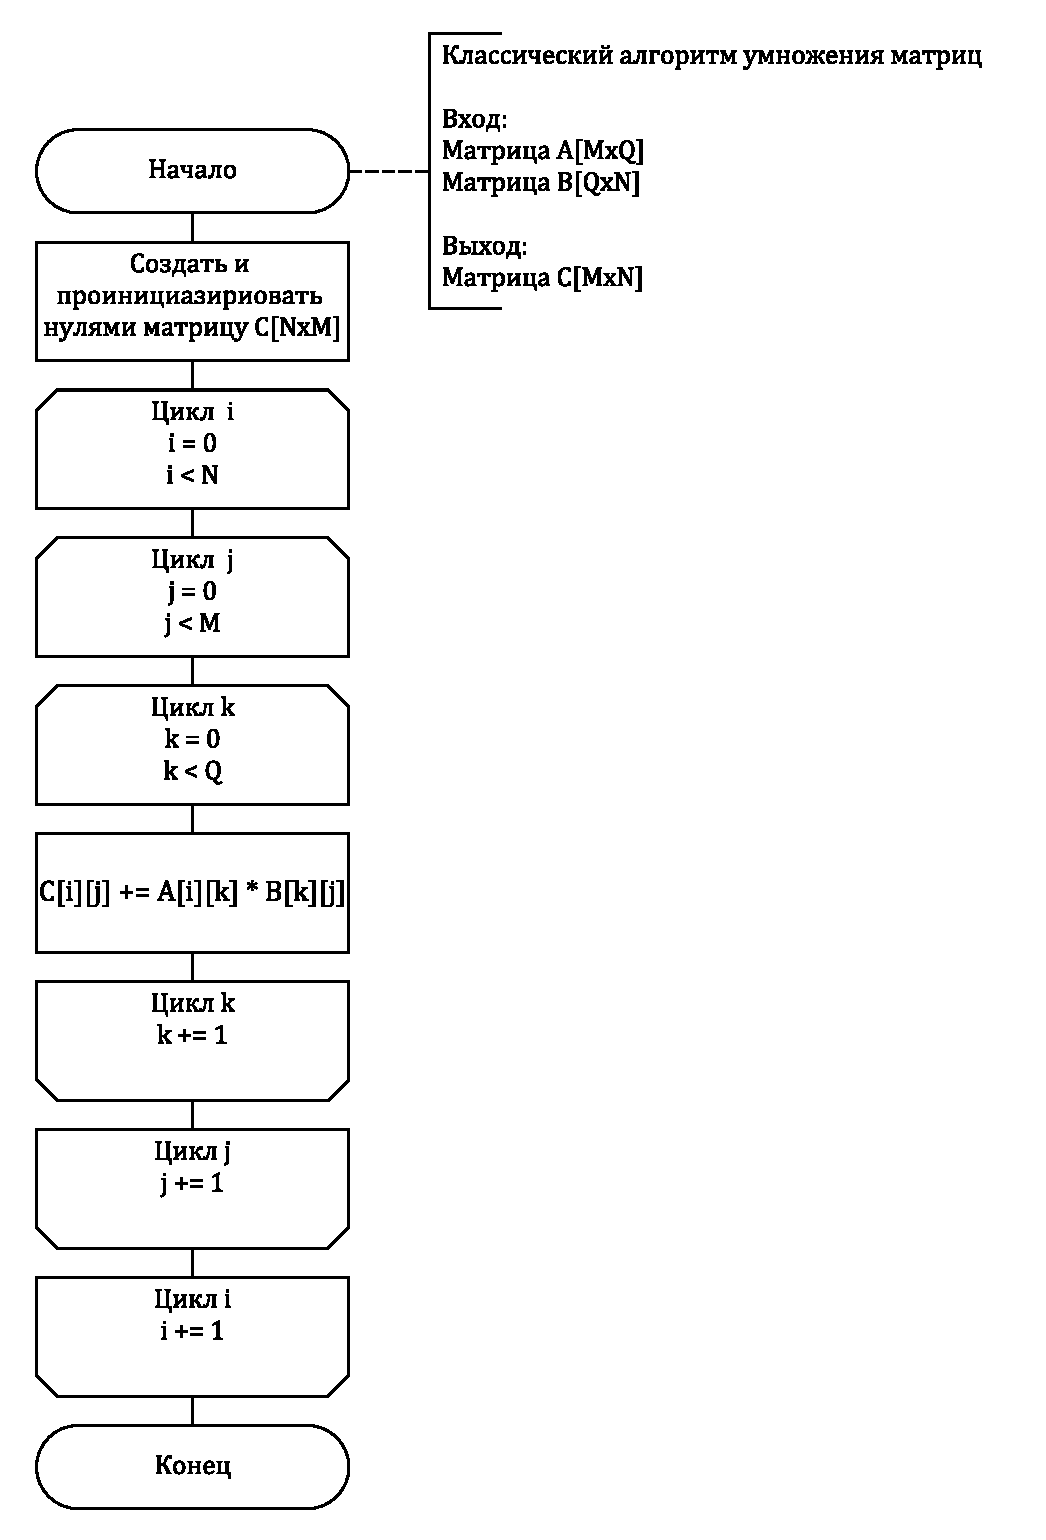
\includegraphics[height=0.65\textheight]{images/stdMult.pdf}
	\caption{Схема стандартного алгоритма умножения матриц}
	\label{img:stdMult}
\end{figure}
\clearpage

\subsection{Разработка алгоритма Винограда для умножения матриц}

На рисунке~\ref{img:WinMult} приведена схема алгоритма Винограда для умножения матриц.

\begin{figure}[H]
	\centering
	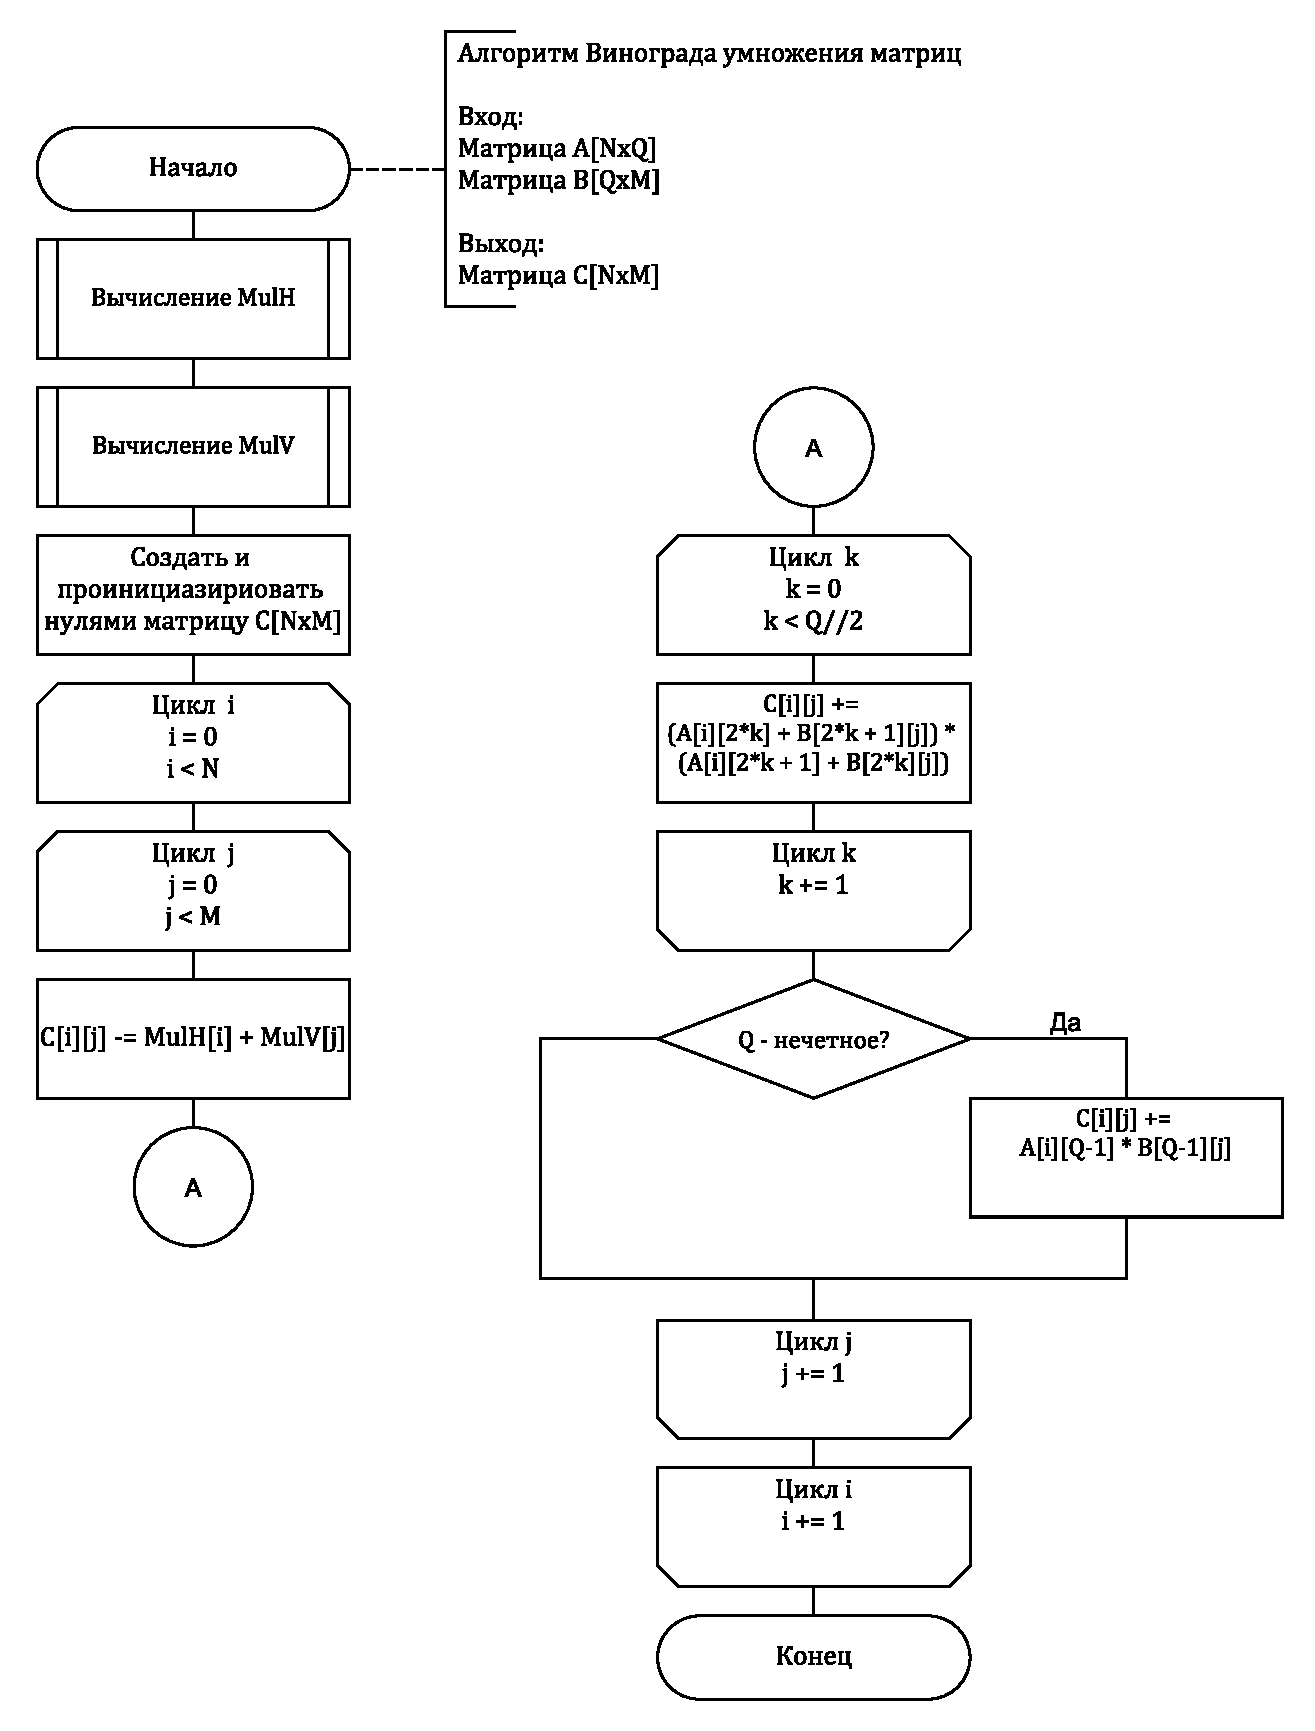
\includegraphics[height=0.8\textheight]{images/WinMult.pdf}
	\caption{Схема алгоритма Винограда для умножения матриц}
	\label{img:WinMult}
\end{figure}
\clearpage

На рисунке~\ref{img:MulH} приведена схема подпрограммы вычисления массива MulV cумм произведений пар соседних элементов строк матрицы.

\begin{figure}[H]
	\centering
	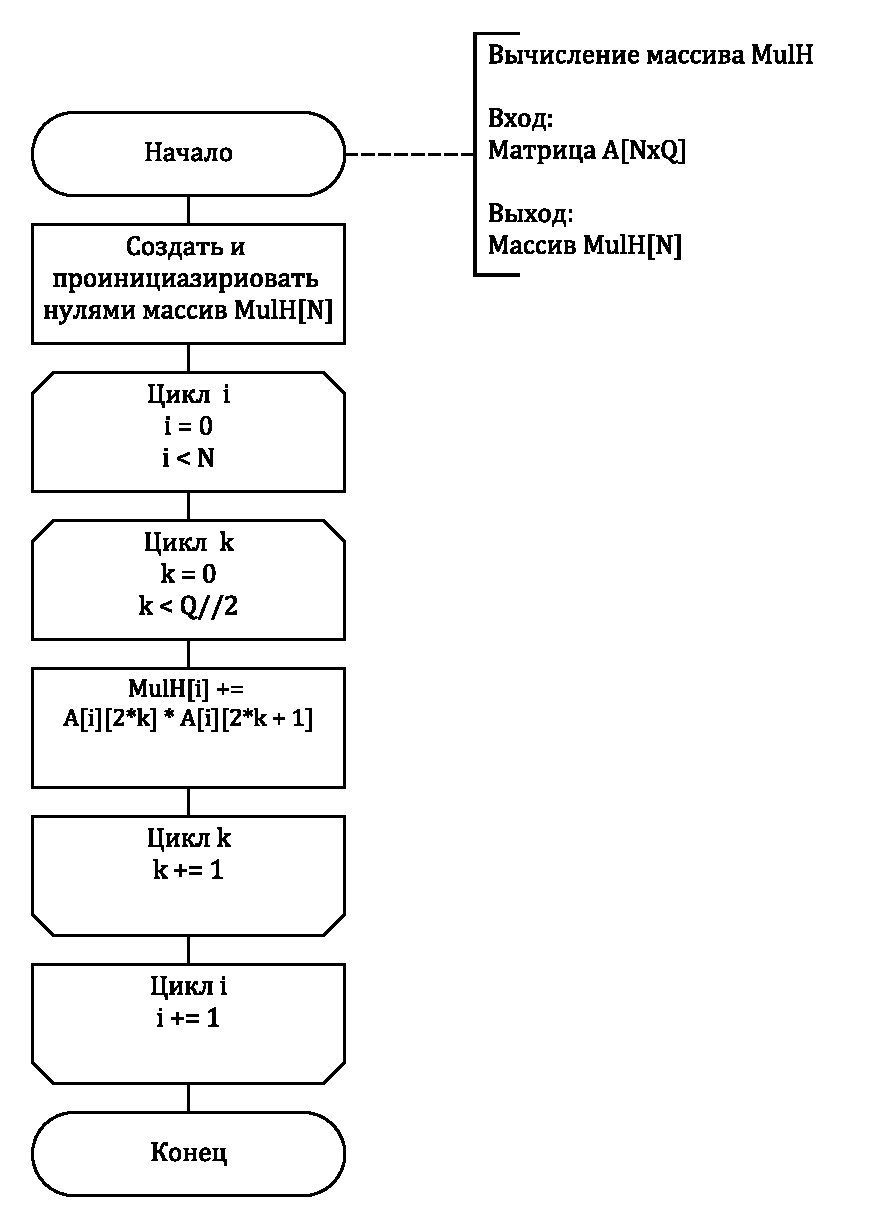
\includegraphics[width=0.7\textwidth]{images/MulH.pdf}
	\caption{Схема подпрограммы вычисления массива MulV cумм произведений пар соседних элементов строк матрицы}
	\label{img:MulH}
\end{figure}
\clearpage

На рисунке~\ref{img:MulV} приведена схема подпрограммы вычисления массива MulH cумм произведений пар соседних элементов колонн матрицы.

\begin{figure}[H]
	\centering
	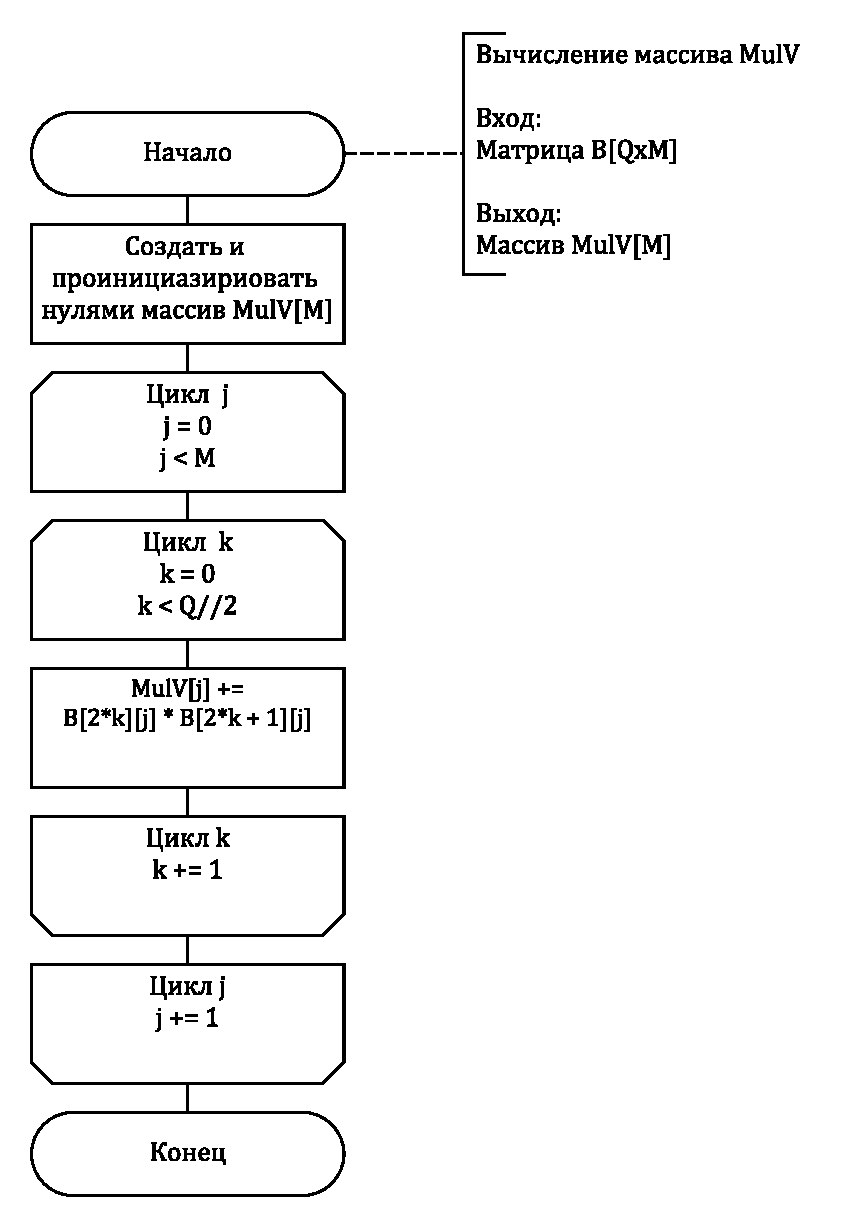
\includegraphics[width=0.7\textwidth]{images/MulV.pdf}
	\caption{Схема подпрограммы вычисления массива MulH cумм произведений пар соседних элементов колонн матрицы}
	\label{img:MulV}
\end{figure}
\clearpage

\subsection{Оптимизация алгоритма Винограда}

На рисунке~\ref{img:WinMultOpt} приведена схема оптимизированного алгоритма Винограда для умножения матриц.

\begin{figure}[H]
	\centering
	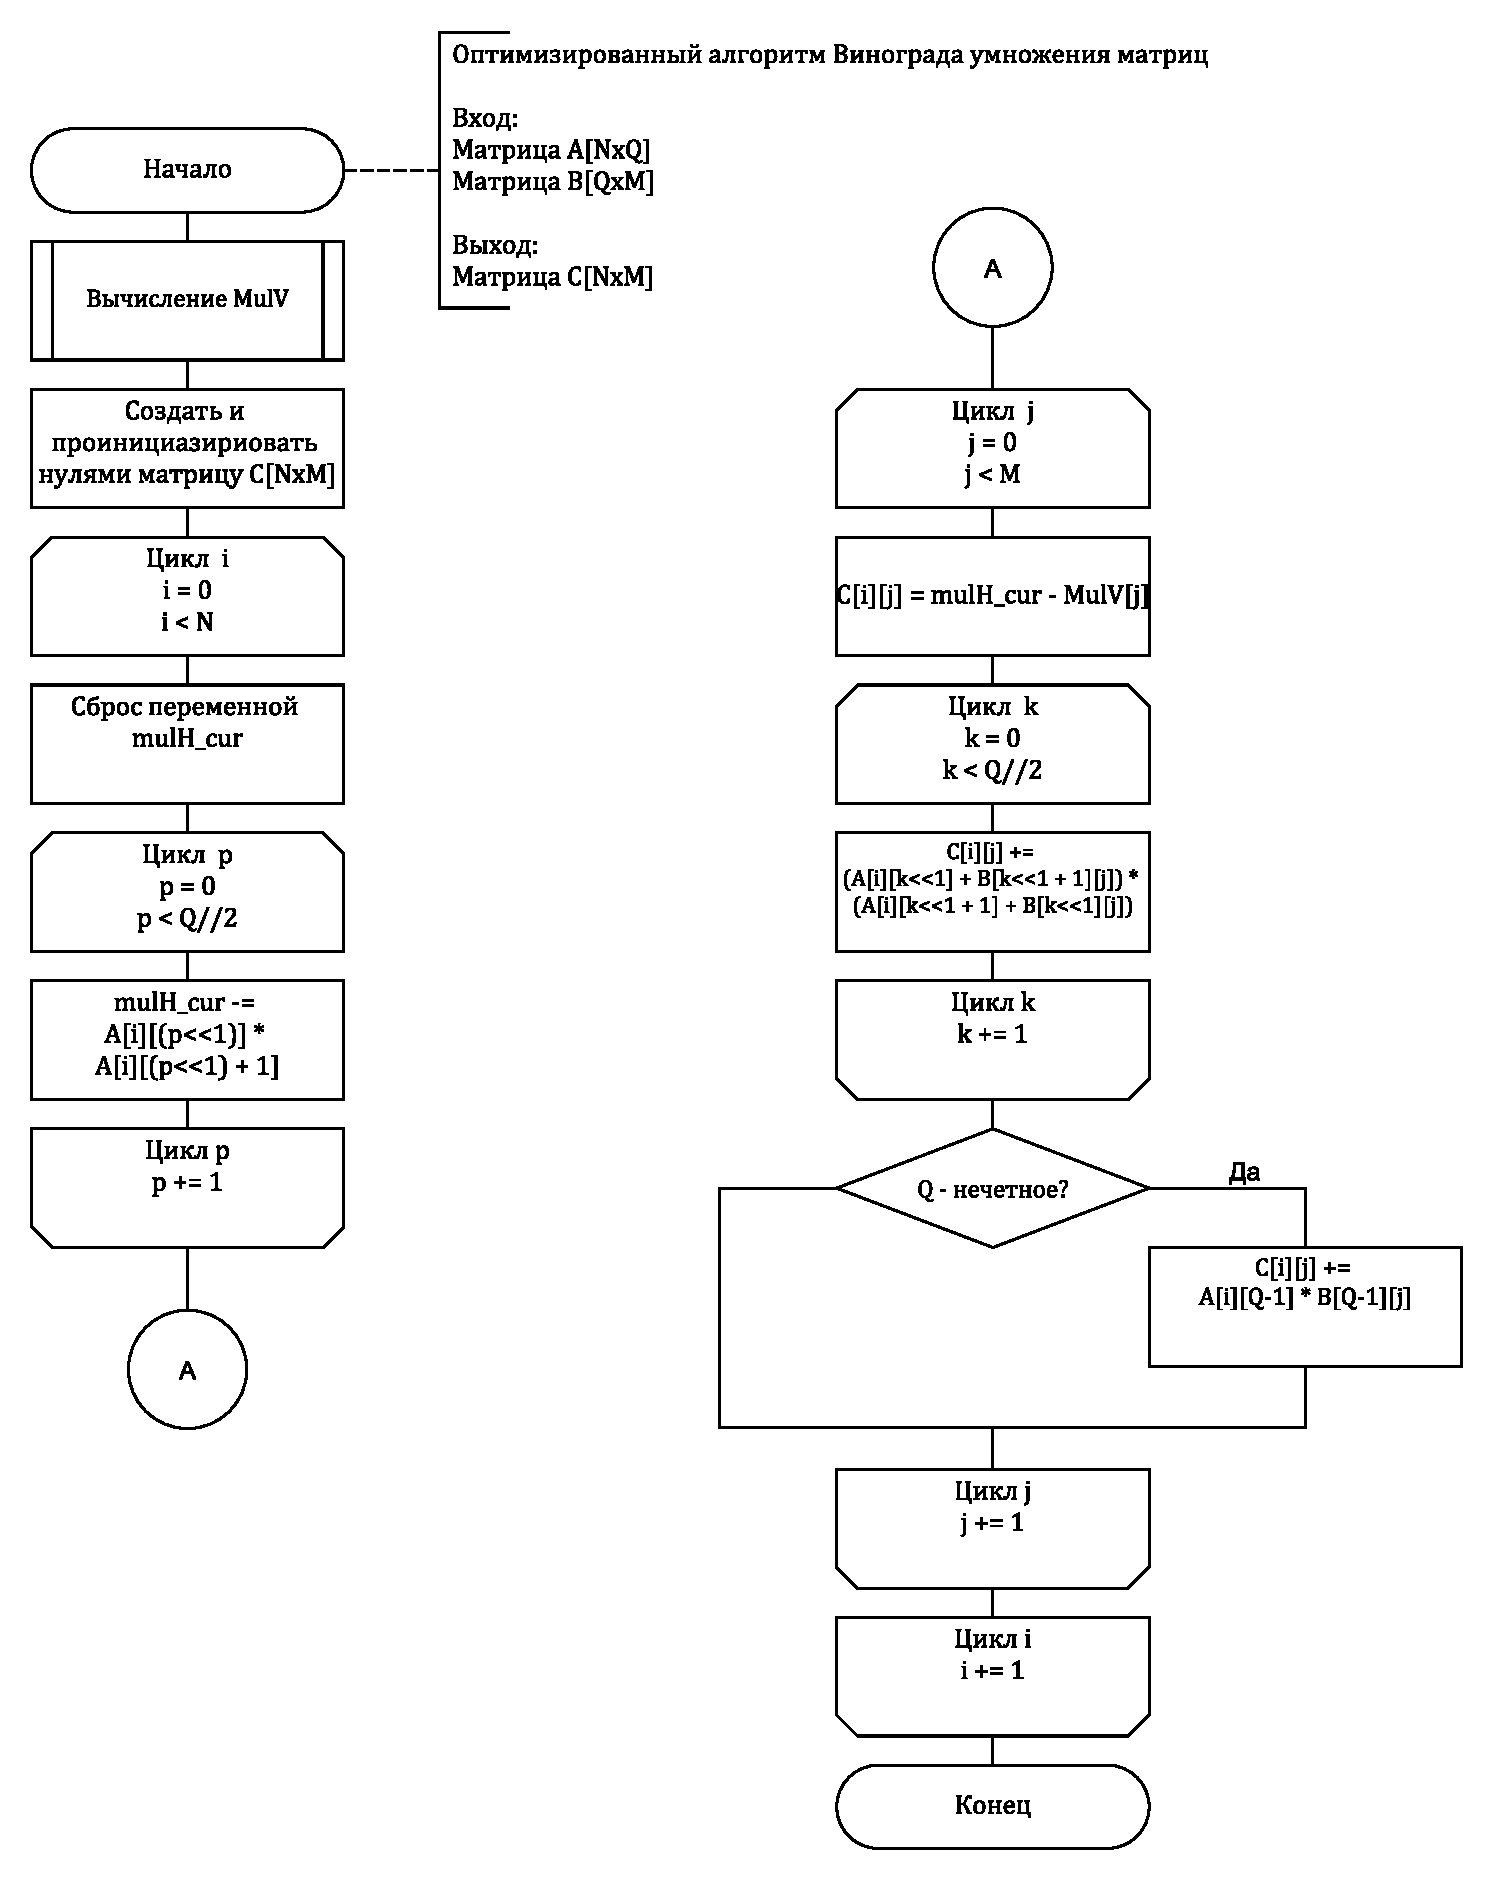
\includegraphics[height=0.8\textheight]{images/WinMultOpt.pdf}
	\caption{Схема оптимизированного алгоритма Винограда для умножения матриц}
	\label{img:WinMultOpt}
\end{figure}
\clearpage

\section{Оценка трудоёмкости алгоритмов}

\subsection{Модель вычислений для оценки трудоёмкости}

Была введена модель вычислений для определения трудоёмкости каждого отдельного взятого алгоритма сортировки.

\begin{enumerate}[label={\arabic*)}]
	\item Трудоёмкость базовых операций имеет:
	\begin{itemize}[label=---]
		\item равную 1:
		\begin{equation}
			\label{for:operations_1}
			\begin{gathered}
				+, -, =, +=, -=, ==, !=, <, >, <=, >=, [], ++, {-}-,\\
				\&\&, >>, <<, ||, \&, |
			\end{gathered}
		\end{equation}
		\item равную 2:
		\begin{equation}
			\label{for:operations_2}
			*, /, \%, *=, /=, \%=
		\end{equation}
	\end{itemize}
	\item Трудоёмкость условного оператора:
	\begin{equation}
		\label{for:if}
		f_{if} = f_{\text{условия}} + 
		\begin{cases}
			min(f_1, f_2), & \text{лучший случай}\\
			max(f_1, f_2), & \text{худший случай}
		\end{cases}
	\end{equation}
	\item Трудоёмкость цикла:
	\begin{equation}
		\label{for:for}
		\begin{gathered}
			f_{for} = f_{\text{инициализация}} + f_{\text{сравнения}} + M_{\text{итераций}} \cdot (f_{\text{тело}} +\\
			+ f_{\text{инкремент}} + f_{\text{сравнения}})
		\end{gathered}
	\end{equation}
	\item Трудоёмкость передачи параметра в функции и возврат из функции равны 0.
\end{enumerate}
\clearpage

\subsection{Трудоёмкость стандартного алгоритма умножения матриц}

Суммарная трудоёмкость $f_{std}$ складывается из трудоёмкостей инициализации матрицы $C_{N \times M}$ ($f_{init}$) и  вложенного цикла ($f_{for}$)

Трудоёмкость инициализации матрицы указана в формуле~\eqref{equ:complexity:std:init};

\begin{equation}
	\label{equ:complexity:std:init}
	f_{init} = 1 \cdot (N \cdot M) = NM
\end{equation}

Трудоёмкость тройного цикла указана в формуле~\eqref{equ:complexity:std:for}

\begin{equation}
	\label{equ:complexity:std:for}
	\begin{gathered}
		f_{for} = 2 + N \cdot(2 + 2 + M\cdot (2 + 2 + Q \cdot (2 + 9))) = 2 + 4N + 4MN + 11MNQ
	\end{gathered}
\end{equation}

Тогда суммарная трудоёмкость находится как сумма~\eqref{equ:complexity:std:init}~+~\eqref{equ:complexity:std:for} и указана в формуле~\eqref{equ:complexity:std}

\begin{equation}
	\label{equ:complexity:std}
	\begin{gathered}
		f_{std} = f_{init} + f_{for} = 11QNM + 5MN + 4N + 2 \approx 11MNQ = O(n^3)
	\end{gathered}
\end{equation}
\clearpage

\subsection{Трудоёмкость алгоритма Винограда умножения двух матриц}

Суммарная трудоёмкость $f_{Win}$ складывается из трудоёмкостей инициализации матрицы $C_{N \times M}$ ($f_{init}$), расчёта массивов MulH и MulV ($f_{mulH}$ $f_{mulV}$ соответственно), и трудоёмкости вложенного цикла ($f_{for}$)

Трудоёмкость инициализации матрицы указана ранее в формуле~\eqref{equ:complexity:std:init};

Трудоёмкость расчёта MulH указана в формуле~\eqref{equ:complexity:Win:mulH};

\begin{equation}
	\label{equ:complexity:Win:mulH}
	\begin{gathered}
		f_{mulH} = N + 2 + N\cdot(2 + (4 + \frac{Q}{2} \cdot (4 + 13))) = 2 + 7N + \frac{17NQ}{2}
	\end{gathered}
\end{equation}

Трудоёмкость расчёта MulV (с учётом оптимизации умножения) указана в формуле~\eqref{equ:complexity:Win:mulV};

\begin{equation}
	\label{equ:complexity:Win:mulV}
	\begin{gathered}
		f_{mulH} = M + 2 + M\cdot(2 + (4 + \frac{Q}{2} \cdot (4 + 13))) = 2 + 7M + \frac{17MQ}{2}
	\end{gathered}
\end{equation}

Трудоёмкость цикла $f_{for}$ указана в формуле~\eqref{equ:complexity:Win:for};

\begin{equation}
	\label{equ:complexity:Win:for}
	\begin{gathered}
		f_{for} = 2 + N\cdot (2 + (2 + M\cdot (2 + (6 + 4 + \frac{Q}{2}\cdot (4 + 25) + 3 +
		\begin{cases}
			0, & \text{Q --- чётное},\\
			11, & \text{иначе}
		\end{cases})))) = \\
		2 + 4N + 15MN + \frac{29MNQ}{2} +
		\begin{cases}
			0, & \text{Q --- чётное},\\
			11MN, & \text{иначе}
		\end{cases}
	\end{gathered}
\end{equation}

Суммарная трудоёмкость находится как сумма~\eqref{equ:complexity:std:init}~+~\eqref{equ:complexity:Win:mulV}~+~\eqref{equ:complexity:Win:mulH}~+~\eqref{equ:complexity:Win:for} и приведена в формуле~\eqref{equ:complexity:Win}

\begin{equation}
	\label{equ:complexity:Win}
	\begin{gathered}
		f_{Win} = f_{init} + f_{mulH} + f_{mulV} + f_{for} = \\
		6 + 7M + 11N + \frac{17MQ}{2} + \frac{17NQ}{2} + 16MN + \frac{29MNQ}{2} +
		\begin{cases}
			0, & \text{Q --- чётное},\\
			11MN, & \text{иначе}
		\end{cases} \\
		\approx \frac{29MNQ}{2} = O(n^3)
	\end{gathered}
\end{equation}
\clearpage

\subsection{Трудоёмкость оптимизированного алгоритма Винограда умножения двух матриц}

Суммарная трудоёмкость $f_{optimized \textunderscore Win}$ складывается из трудоёмкости инициализации матрицы $C_{N \times M}$ ($f_{init}$), трудоёмкости расчёта массива MulV ($f_{mulV}$), и трудоёмкости вложенного цикла ($f_{for}$)

Трудоёмкость инициализации матрицы указана ранее в формуле~\eqref{equ:complexity:std:init};

Трудоёмкость расчёта MulV (с учётом оптимизации умножения) указана в формуле~\eqref{equ:complexity:Win:mulV};

\begin{equation}
	\label{equ:complexity:optWin:mulV}
	\begin{gathered}
		f_{mulV} = M + 2 + M\cdot(2 + (4 + \frac{Q}{2} \cdot (4 + 11))) = 2 + 7M + \frac{15MQ}{2}
	\end{gathered}
\end{equation}

Трудоёмкость цикла $f_{for}$ указана в формуле~\eqref{equ:complexity:optWin:for};

\begin{equation}
	\label{equ:complexity:optWin:for}
	\begin{gathered}
		f_{for} = 2 + N \cdot (7 + \frac{Q}{2}\cdot(4 + 10) + (2 + M \cdot (2 + 12 + \frac{Q}{2} \cdot (4 + 21) + 
		\begin{cases}
			0, & \text{Q --- чётное},\\
			11MN, & \text{иначе}
		\end{cases}))) = \\
		2 + 9N + 7NQ + 14MN + \frac{25MNQ}{2} +
		\begin{cases}
			0, & \text{Q --- чётное},\\
			11MN, & \text{иначе}
		\end{cases}
	\end{gathered}
\end{equation}

Суммарная трудоёмкость находится как сумма~\eqref{equ:complexity:std:init}~+~\eqref{equ:complexity:optWin:mulV}~+~\eqref{equ:complexity:optWin:for} и приведена в формуле~\eqref{equ:complexity:optWin}

\begin{equation}
	\label{equ:complexity:optWin}  
	\begin{gathered}
		f_{optimised \textunderscore Win} = f_{init} + f_{mulV} + f_{for} = \\
		4 + 7M + 9N + 7NQ + \frac{15MQ}{2} + 15MN + \frac{25MNQ}{2} +
		\begin{cases}
			0, & \text{Q --- чётное},\\
			11MN, & \text{иначе}
		\end{cases} \\
		\approx \frac{25MNQ}{2} = O(n^3)
	\end{gathered}
\end{equation}

\section*{Вывод}

В данном разделе были построены схемы алгоритмов умножения матриц, рассматриваемых в лабораторной работе, введена модель вычислений и проведена теоретическая оценка трудоёмкости представленных алгоритмов. Согласно приведённой оценке, трудоёмкость стандартного алгоритма Винограда на 21\% больше, чем у его оптимизированной версии, и на 32\% больше трудоёмкости стандартного алгоритма в введённой модели вычислений.

\clearpage
